\documentclass[12pt,xcolor=dvipsnames]{beamer}
\usetheme{CambridgeUS}
\usecolortheme{whale}
\setbeamercolor{block title}{use=structure,fg=white,bg=blue!75!black}  
\setbeamercolor{block body}{use=structure,fg=black,bg=blue!5!white}
\setbeamercolor{frametitle}{bg=Blue}

\usepackage{hyperref}   
\usepackage{url}
\hypersetup{urlcolor=red}

\renewcommand{\bibname}{References}
\setbeamertemplate{bibliography item}{[\theenumiv]}

\usepackage{multicol}
\usepackage{verbatim} 
\usepackage{graphics}
\usepackage{graphicx}


%Basic Information
\title{Study and Integration of edX InSight}
\author{Sagar Agarwal}
\date{\today}

%--------------------------------------------------------------------------------------
%               TITLE PAGE (Slide 1)
%--------------------------------------------------------------------------------------
\begin{document}
\begin{frame}
\titlepage
\end{frame}
%--------------------------------------------------------------------------------------


%--------------------------------------------------------------------------------------
%               Outline
%--------------------------------------------------------------------------------------
\begin{frame}
\frametitle{Outline}
\begin{multicols}{2}
\tableofcontents[hideallsubsections]
\end{multicols}
\end{frame}

%--------------------------------------------------------------------------------------
%               Slide 1: Topic 1
%--------------------------------------------------------------------------------------
\section{Motivation for the  Project}
\begin{frame}[t]
\frametitle{Motivation for the  Project}
%Write text here. \\
%This is the first slide

%For bulleted points use the following:\\
\begin{itemize}
 \item Education
 \item Business
 \item Health
 \item Administrative
\end{itemize}

%For numbered list use the following:\\
%\begin{enumerate}
 %\item write point 1
 %\item write point 2
%\end{enumerate}

\end{frame}

%--------------------------------------------------------------------------------------
%               Slide 2: Subtopic of Topic 1
%--------------------------------------------------------------------------------------

\subsection{Education}
\begin{frame}[t]
\frametitle{Educational Perspective}

\begin{center}
%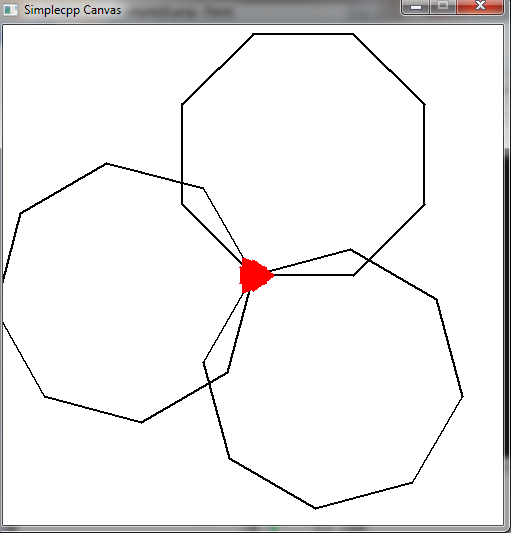
\includegraphics[height=3.5cm]{simple19.png}\\ % Insert your image it this way
%Fig: SimpleCPP Output \cite{SimpleCPP-Windows}
\subsection{Course Enhancement}
\begin{center}
\textit{Course Enhancement}

\end{center}
\begin{center}
Analysis of time required and performance on particular test can give information about the understanding level of students and the difficulty level of test.\\

It  can also give information about difficulty level of course and hence instructor can enhance course content
\end{center}

\end{center}
\end{frame}

%--------------------------------------------------------------------------------------
%               Slide 3: Subtopic of Topic 1
%--------------------------------------------------------------------------------------

\subsection{Business}
\begin{frame}[t]
\frametitle{Business Perspective}

\begin{center}
%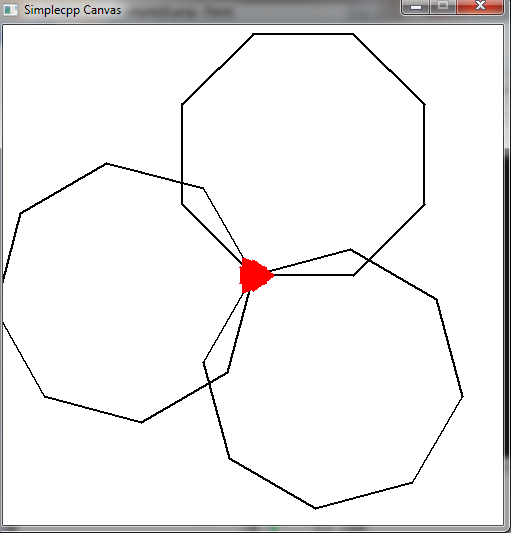
\includegraphics[height=3.5cm]{simple19.png}\\ % Insert your image it this way
%Fig: SimpleCPP Output \cite{SimpleCPP-Windows}
\subsection{Predictive analytics }
\begin{center}

\end{center}
\textit{Predictive analytics}

\end{center}
\begin{center}


Stores can use  data to  analyse past buying behaviour to predict the coupons or promotions a customer is most to participate in or buy in the future. Predictive analytics could also be applied to customer website browsing behaviours to deliver a personalized website experience for the customer.
\end{center}

\end{frame}
%--------------------------------------------------------------------------------------
%               Slide 4: Subtopic of Topic 1
%--------------------------------------------------------------------------------------

\subsection{Health}
\begin{frame}[t]
\frametitle{Health Perspective}

\begin{center}
%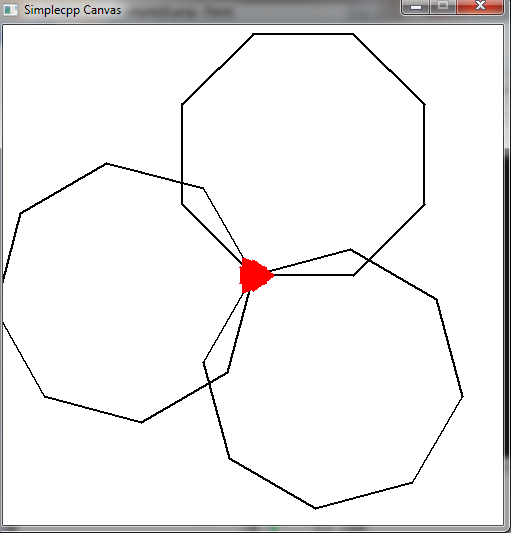
\includegraphics[height=3.5cm]{simple19.png}\\ % Insert your image it this way
%Fig: SimpleCPP Output \cite{SimpleCPP-Windows}
\subsection{Personalized Medicine }
\begin{center}

\end{center}
\textit{Personalized Medicine}

\end{center}
\begin{center}


With human genome mapping and Big Data tools, it will soon be commonplace for everyone to have their genes mapped as part of their medical record. This brings medicine closer than ever to finding the genetic determinants that cause a disease and developing drugs expressly tailored to treat those causes — in other words, personalized medicine.
\end{center}

\end{frame}
%--------------------------------------------------------------------------------------
%               Slide 5: Subtopic of Topic 1
%--------------------------------------------------------------------------------------

\subsection{Administration}
\begin{frame}[t]
\frametitle{Administrative Perspective}

\begin{center}
%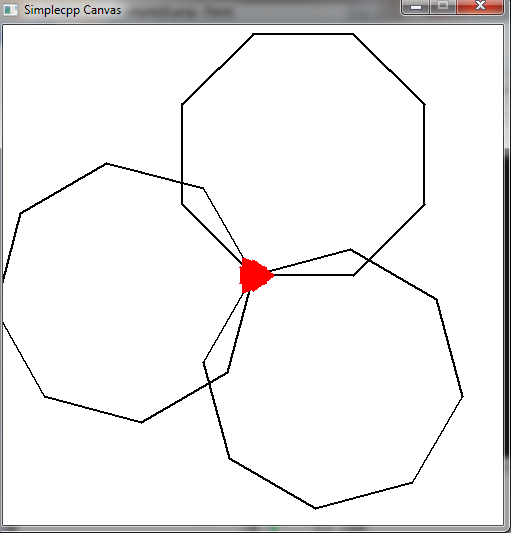
\includegraphics[height=3.5cm]{simple19.png}\\ % Insert your image it this way
%Fig: SimpleCPP Output \cite{SimpleCPP-Windows}
\subsection{Administrative Perspective }




\textit{Providing better Environment}






Big data can provide information about traffic flow in various parts of city during various time periods .
This data can be used to optimize timings of traffic signals which can reduce $CO_2$ emission .



\end{center}
\end{frame}

\end{document}